\documentclass[article]{report}

\usepackage[T1]{fontenc}
\usepackage[utf8]{inputenc}
\usepackage{latexsym}
\usepackage[francais]{babel}
\usepackage{url}
\usepackage{geometry}
\geometry{tmargin=2.5cm, bmargin=2.4cm, lmargin=3cm, rmargin=2cm}
\usepackage{graphicx}
\usepackage[footnote, nolist]{acronym}
\usepackage{pdfpages}
\usepackage{newcent}
\usepackage{color}
\usepackage{listings}
\usepackage{tikz}
\usepackage{ifthen}
\usepackage{wrapfig}
\usepackage{textcomp}
\usepackage{multicol}
\setlength{\columnsep}{1cm}

\bibliographystyle{apalike}
\parskip = 0.25cm

%
% Document
%
\begin{document}
		\thispagestyle{empty}
  			\begin{titlepage} 
						\vspace*{5cm} 
  					\begin{center} 
  							{\huge{\textsc{Cahier des charges} \\ ~ \\{\large From}\\ ~\\ Team Dedalus \\ ~ \\ Islands}}
	  						\vspace*{11cm}
						\end{center}
  					\hfill {\large Romain \textsc{Biessy}}
  					\hfill {\large Renaud \textsc{Gaubert}}
  					\hfill {\large Aenora \textsc{Tye}}
  					\hfill {\large Erwan  \textsc{Vasseure}}
  			\end{titlepage} 
  	\renewcommand{\contentsname}{Sommaire}

  	\tableofcontents
  			\newpage
				\title{Introduction}%<- modifier la pagination
								Even though we didn't start coding, we still had six to seven group meeting to discuss about the project. And spent at least 15 hours speeking together.\newline
								However, the project's general gameplay was fixed unanimously on the first reunion. It will be a 3D RTS at the first person. Thus a mix between RTS and FPS. Creating a game has never been an easy task but, the game how we see could be described as ambitious. Nevertheless, our teamwork should not be underestimate.\\
								
								When we assigned the differents task to our members, we had in mind the idea that everybody should know how most of the game works and not only one member. Therfore, we had to split the project in a way that would help us later : modules. Thus even if we didn't begin to code the game, we have some kind of base. 								
								
				\part{Project presentation}
      			\chapter{Gameplay}
								\section{Section 1}
									  \subsection{Sub 1}
						\chapter{Goals and interest}
								\section{Learning}
										Since half of the group are inexperienced programmers, one of the major goal of the project will be to learn about computer programming.\newline
										Of course it won't be limited to C\#, because of the fact that we are working with OO, to ensure that everybody can understand the code, we will be using UML.\newline
										Also we will have to use XMl with the GUI
									  \subsection{Sub 1}
     		\part{What must be done}
     			\chapter{Behind the scene}
     					\section{Language \& Game design pattern}
     						Our project will be coded in \textbf{C\#} .NET 4.0 mainly because of the \ac{OOP} paradigm and also for the large choice there is about 3d engine and libraries. The OO let us use the \textbf{game state} pattern in order to structure the code. Basically, we consider our game as a stack of different states. Here is an example of a game state:\newline
     						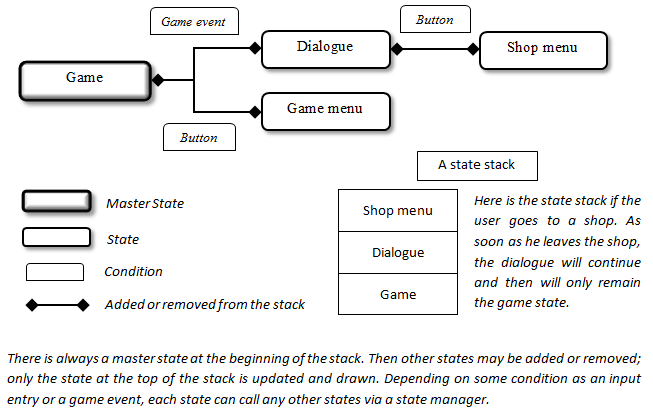
\includegraphics[height=300px]{GameStateDesign.png}\\
     						
     						This pattern is advised for \ac{RTS} games, among others. As we are working in a group, it is important to keep homogeneity throughout the program. Besides, a well-structured code will be easier to understand and to edit.
					\section{3D Engine \& Library}
						The 3d engine we will use is \textbf{\ac{Mogre}}. Initially, this is an \ac{API} coded in C++ called Ogre; Mogre is an advanced .NET 2.0 wrapper for Ogre. We have chosen this \ac{API} since it is known as an effective, handy and well-documented 3D engine in C\#.\\			
						Our \ac{GUI} will be implemented with the library \textbf{\ac{MyGUI}}. It’s very flexible since all parameters are settable directly in the XML’s files.\\	
						Since our 3D engine doesn’t handle sound we have to use an audio library. We will use \textbf{NAudio} - an open source .NET library - because of its simplicity and completeness.
					\section{Softwares}
						Our \ac{IDE} will be \textbf{Visual Studio 2010 Ultimate}. We will also need \textbf{Blender} so that we can create our own meshes and then use them for our game with the script Blender2Ogre. Basically, all of our 3D objects will be created with Blender except for the terrain’s cubes which are generated directly in the source code.
					\section{Algorithm}
						There are two key points in our projects which will have to be implemented using some well-known algorithms:
						
						\begin{itemize}
\renewcommand{\labelitemi}{$\bullet$}
\item \textbf{Terrain generation}. We want our land to be generated pseudo-randomly in order to create realistic islands - apart the fact that they are suspended in the sky. We want our islands to have mountains, jungles and rivers but we will definitely not build them ourselves. What we need to implement is the algorithm of \textbf{Perlin noise} in 3 dimensions. The idea for one dimension is to generate a list of random points, then to create a function which goes through these points. We repeat this step many times with an amplitude between the points getting smaller and smaller and then we add all the functions obtained. The concept is the same in 3 dimensions.\\

\item \textbf{Pathfinding}. This is part of the \ac{AI} for the \ac{NPC}. The goal is to find the shortest way from a point A to a point B. A common solution for this problem is the \textbf{(A*)} algorithm. Basically, it tests all possibilities of path and then remembers the path which is getting closer to the arrival. This method is efficient and quick as long as there is no intricate labyrinth that’s why we think (A*) is adapted for our project.
\end{itemize}

\begin{acronym}
\acro{OOP}{Oriented-Object Programming}
\acro{RTS}{Real Time Strategy}
\acro{Mogre}{Managed Ogre}
\acro{API}{Application Progamming Interface}
\acro{GUI}{Graphical User Interface}
\acro{MyGUI}{Multilayer and overlappable GUI System}
\acro{IDE}{Integrated Developement Environment}
\acro{AI}{Artificial Intelligence}
\acro{NPC}{Non Player Character}
\end{acronym}
     		
\end{document}
